%\documentclass[12pt]{amsart}
%\RequirePackage{luatex85}
\documentclass{hipatia}
\usepackage[brazil]{babel}
\usepackage[utf8]{inputenc}
\usepackage{amscd}
\usepackage{amsfonts}
\usepackage{amsgen}
\usepackage{amsmath}
\usepackage{amssymb}
\usepackage{amstext}
\usepackage{amsthm}
\usepackage{graphicx}
\usepackage{indentfirst}
\usepackage{enumitem}
\usepackage{latexsym}
\usepackage{makeidx}
%\usepackage{index}
%\usepackage{pictexwd}
\usepackage{epsfig}
\usepackage{wrapfig}
%\usepackage[all,knot,arc,import,poly]{xy}
%\usepackage[usenames]{color}

\usepackage[mathscr]{eucal}
\usepackage[T1]{fontenc}
%\usepackage{ae}
\usepackage{parskip}%------------------------>remove identação
\usepackage{fancybox}%------------------------>permite inserir caixa oval
\usepackage{tcolorbox}%------------------------>colorir caixa de teorema
\tcbuselibrary{theorems}%------------------------>colorir caixa de teorema
\usepackage{hyperref}

%%%%%%%%%%%%%%%%% DEFINIÇÕES %%%%%%%%%%%%%%%%
\newtheorem{Df}{Definição}
%[section]
\newtheorem{Teo}[Df]{Teorema}
\newtheorem{Prop}[Df]{Proposição}
\newtheorem{Lem}[Df]{Lema}
\newtheorem{Ex}[Df]{Exemplo}
\newtheorem{Exs}[Df]{Exemplos}
\newtheorem{Obs}[Df]{Observação}
\newtheorem{Fat}[Df]{Fato}
\newtheorem{Que}[Df]{Questão}
\newtheorem{Cor}[Df]{Corolário}

%% Sugestão de macros: por Samuel e João Paulo %%
\newcommand{\fp}{\hfill{$\square$}}
\newcommand{\fd}{\hfill{$\blacksquare$}}
\newcommand{\fo}{\hfill{$\triangle$}}
\newcommand{\bc}{\begin{center}}
\newcommand{\ec}{\end{center}}
\newcommand{\n}{\noindent}
\newcommand{\dem}{\n{\bf Demonstração: }}
\newcommand{\pr}{\n{\bf Prova: }}
\newcommand{\N}{\mathbb{N}}
\newcommand{\Z}{\mathbb{Z}}
\newcommand{\Q}{\mathbb{Q}}
\newcommand{\R}{\mathbb{R}}
\newcommand{\C}{\mathbb{C}}

%%%%%%%%%%%%
\newcommand{\sn}[1][n]{\ensuremath{S_{{#1}}}}
\newcommand{\St}[1][2]{\ensuremath{\mathbb S}^{#1}}
\newcommand{\brak}[1]{\ensuremath{\left\{ #1 \right\}}}
\newcommand{\ang}[1]{\ensuremath{\left\langle #1\right\rangle}}
\newcommand{\set}[2]{\ensuremath{\left\{#1 \,\mid\, #2\right\}}}
\newcommand{\reth}[1]{Theorem~\protect\ref{th:#1}}
\newcommand{\relem}[1]{Lemma~\protect\ref{lem:#1}}
\newcommand{\repr}[1]{Proposition~\protect\ref{prop:#1}}
\newcommand{\reco}[1]{Corollary~\protect\ref{cor:#1}}
\newcommand{\req}[1]{equation~(\protect\ref{eq:#1})}

\makeatletter
\def\@map#1#2[#3]{\mbox{$#1 \colon\thinspace #2 \to #3$}}
\def\map#1#2{\@ifnextchar [{\@map{#1}{#2}}{\@map{#1}{#2}[#2]}}
\makeatother

%%%%%%%%%%%
\newcommand{\vsete}{\vspace*{0.7cm}}
\newcommand{\vcinco}{\vspace*{0.5cm}}
\newcommand{\vtres}{\vspace*{0.3cm}}
\newcommand{\vum}{\vspace*{0.1cm}}
\newcommand{\no}{\noindent}


%\input{xypic}
%%	Caminho das imagens	 %%
\graphicspath{}
%%	Novos Teoremas	%%
\newtheorem{teo}{Teorema}[section]
\newtheorem{lem}[teo]{Lema}
\newtheorem{defi}[teo]{Definição}
\newtheorem{obs}[teo]{Observação}
\newtheorem{prop}[teo]{Proposição}
\newtheorem{cor}[teo]{Corolário}
\newtheorem{exe}[teo]{Exemplo}
\newtheorem{fato}[teo]{Fato}
\newtheorem*{axiesc}{$(\ac)$ Axioma da Escolha}
\newtheorem*{axiinf}{Axioma do Infinito}
\newtheorem*{jus}{Justificativa}
\newtheorem*{dmt}{Demonstração}
\newtheorem*{ideia}{Ideia da prova}
\newtcbtheorem[number within=section]{teoremacaixa}{}%
{colback=white!35,colframe=yellow!10!black!,fonttitle=\bfseries}{th}%------------------------>Teorema na caixa

%%	Novos Comandos	%%

\newcommand{\equip}{\approx}

\newcommand{\preord}{\mathbb{P}}
\newcommand{\preordem}{\langle \preord, \le \rangle}
\newcommand{\bound}[1]{\mathfrak{b}(#1)}
\newcommand{\domin}[1]{\mathfrak{d}(#1)}
\newcommand{\Ideal}{\mathcal{I}}
\newcommand{\Filt}{\mathcal{F}}
\newcommand{\Ip}{\mathcal{I}_\preord}
\newcommand{\bP}{\bound{\preord}}
\newcommand{\dP}{\domin{\preord}}
\newcommand{\PV}{\mathcal{PV}}
\newcommand{\Cat}{\mathcal{C}}
\newcommand{\Morph}[3]{#1 \xrightarrow{\quad #2 \quad} #3}
\newcommand{\dts}{\dial_2(\textbf{Sets})}
\newcommand{\dualr}[1]{\mathrel{#1}^*}
\newcommand{\partes}[1]{\mathcal{P}(#1)}

\usepackage{mathabx}
\usepackage{scalerel}
\usepackage{graphicx}
\newcommand{\nback}[1][-.95pt]{
  \mathrel{\raisebox{#1}{$\rotatebox[origin=c]{-315}{\scaleobj{0.55}{-}}$}}
}
\newcommand{\preccurlyneq}{%
\mathrel{\ooalign{$\preccurlyeq$\cr\kern1.2pt$\nback$}}}

\newcommand{\la}{\langle}
\newcommand{\da}{\rangle}
\newcommand{\B}{\mathcal{B}}
\newcommand{\D}{\mathcal{D}}
\newcommand{\F}{\mathcal{F}}
\newcommand{\G}{\mathcal{G}}
\newcommand{\po}{\mathbb{P}}
\newcommand{\p}{\mathcal{P}}
\newcommand{\U}{\mathcal{U}}
\newcommand{\V}{\mathcal{V}}
\newcommand{\subs}{\subseteq}
\newcommand{\cont}{\supseteq}
\newcommand{\rest}{\upharpoonright}

\newcommand{\cnuum}{\emph{continuum }}
\newcommand{\ch}{\mathbf{CH}}
\newcommand{\wo}{\mathbf{WO}}
\newcommand{\gch}{\mathbf{GCH}}
\newcommand{\continuum}{\mathfrak{c}}
\newcommand{\ac}{\mathbf{AC}}
\newcommand{\zf}{\mathbf{ZF}}
\newcommand{\zl}{\mathbf{ZL}}
\newcommand{\zfc}{\mathbf{ZFC}}
\newcommand{\acw}{\mathbf{AC_\omega}}
\newcommand{\acwfin}{\mathbf{AC_\omega(Fin)}}
\newcommand{\dc}{\mathbf{DC}}
\newcommand{\dcl}{\mathbf{DC'}}
\newcommand{\rs}{\mathbf{RS}}
\newcommand{\cutfin}{\mathbf{CUT(Fin)}}
\newcommand{\on}{\mathbf{On}}

\DeclareMathOperator{\Dom}{dom}
\DeclareMathOperator{\Codom}{cod}
\DeclareMathOperator{\Image}{Im}
\DeclareMathOperator{\Obj}{Obj}
\DeclareMathOperator{\Mor}{Mor}
\DeclareMathOperator{\dial}{Dial}
\DeclareMathOperator{\Fin}{Fin}
\DeclareMathOperator{\Cofin}{Cofin}
\DeclareMathOperator{\Enum}{Enum}
\DeclareMathOperator{\Coenum}{Coenum}

%% Sugestão de macros: por João Paulo %%
\newcommand{\fss}{\hfill{$\triangle$}}


%% comandos da lista de conjuntos

\newcommand{\esp}{\vspace*{0.5cm}}
\newcommand{\esple}{\vspace*{0.3cm}}
\newcommand{\vaz}{\emptyset}
\newcommand{\s}{\subseteq}
\newcommand{\se}{\subset}
\newcommand{\ns}{\not\s}
\newcommand{\nse}{\not\se}
\newcommand{\co}{\supseteq}
\newcommand{\coe}{\supset}
\newcommand{\nco}{\not\coeq}
\newcommand{\ncoe}{\not\co}
%\newcommand{\qc}{\s^*}
\newcommand{\qce}{\s^*}
\newcommand{\nqc}{\not\s^*}
\newcommand{\nqce}{\not\s^*}
\newcommand{\qco}{\coeq^{*}}
\newcommand{\qcoe}{\co^{*}}
\newcommand{\nqco}{\not\coeq^{*}}
\newcommand{\nqcoe}{\not\co^{*}}
\newcommand{\meni}{\leqslant}
\newcommand{\nmeni}{\nleqslant}
\newcommand{\mai}{\geqslant}
\newcommand{\nmai}{\ngeqslant}
\newcommand{\menie}{\leqslant^{*}}
\newcommand{\nmenie}{\not\leqslant^{*}}
\newcommand{\maie}{\geqslant^{*}}
\newcommand{\nmaie}{\ngeqslant^{*}}
\newcommand{\res}{\upharpoonright}
\newcommand{\pe}{\langle}
\newcommand{\pd}{\rangle}
\newcommand{\dominado}{\preccurlyeq}
\newcommand{\ndominado}{\not\preccurlyeq}


%comando dos exercicios de Diego de 2017

\newcommand{\unidis}{\oplus}
\newcommand{\unidisg}{\bigoplus}
\let\widering\relax

\usetikzlibrary{
    positioning, % Para posicionar nós de forma relativa (ex: above=of)
    arrows.meta,  % Para estilos de setas modernos (ex: Latex)
    matrix,  
    backgrounds,
    shapes.geometric
}

\begin{document}
\setcounter{page}{\teoremapage}
\subtitle{Teorema}
\title %[$\gch$ implica $\ac$]
{\fontsize{26}{26}\selectfont A Hipótese Generalizada do Contínuo\\
\fontsize{26}{26}\selectfont Implica o Axioma da Escolha}
\author{Samuel Gomes da Silva e Diego Lima Bomfim
\footnote{O segundo autor teve o apoio da Coordenação de Aperfeiçoamento de Pessoal de Nível Superior - Brasil (CAPES) - Código de Financiamento 001}
}
%\address{Instituto de Matemática e Estatística -- Universidade Federal da Bahia \\ \newline
%av. Milton Santos s/n, Campus Ondina, 40170-110, \newline Salvador/Bahia, Brasil.}
%\email{samuel@ufba.br}
%\email{bomfim.diego@ufba.br}
%\footnote{O segundo autor teve o apoio da Coordenação de Aperfeiçoamento de Pessoal de Nível Superior - Brasil (CAPES) - Código de Financiamento 001\\}

%\begin{abstract}
%    Neste artigo, trabalhamos com o Axioma da Escolha
%  e com a Hipótese do Contínuo, apresentando os seus 
%  contextos conjuntistas e suas notáveis influências 
%  na História da Matemática. Exibimos, com grande 
%  detalhamento,  o sabor dos argumentos combinatórios 
%  com os quais Sierpi\'nski, se valendo do poder 
%  dedutivo da Hipótese Generalizada do Contínuo, 
%  pôde demonstrar a validade do Axioma da Escolha 
%  -- utilizando-se para isso de {\it formas cardinais} 
%  deste último. Como resultado intermediário muito 
%  importante, damos grande destaque \`a principal 
%  entre as formas cardinais do Axioma da Escolha 
%  - a saber, aquela dada pelo célebre teorema 
%  provado por Tarski em 1924: o Axioma da Escolha 
%  é equivalente à asserção ``para todo conjunto infinito 
%  $X$, $X^2$ é equipotente a $X$". 
%\end{abstract}

\maketitle

\section{Introdução}

O Axioma da Escolha surgiu ``oficialmente'' em 1908 a partir
da publicação, por Ernst Zermelo, de dois trabalhos
(\cite{Zer1908,Zer1908a}) que marcaram o início da
axiomatização da {\it Teoria dos Conjuntos}, tendo sido
utilizado pela primeira vez quatro anos antes pelo mesmo
autor em sua demonstração de que todo conjunto pode ser bem
ordenado (\cite{Zer1904}) -- que por sua vez é conhecido como
Teorema da Boa Ordenação (denotado por $\wo$, de {\it
Well-Ordering Theorem}).

Devido ao seu caráter não-construtivo, $\ac$ (como é
geralmente denotado o Axioma da Escolha -- advindo de {\it
Axiom of Choice}) foi, e ainda é, alvo de muita discussão e
polêmica:  afinal, ele garante ao trabalhador matemático a
tentadora possibilidade de fazer infinitas escolhas
arbitrárias. Em termos simples, ele garante que dada uma
família de conjuntos não-vazios sempre é possível obter um
conjunto que tem exatamente um elemento escolhido em cada
conjunto da família, no que se diz que toda família de
conjuntos não-vazios admite uma {\it
função-escolha}\footnote{Uma função-escolha para uma família
$\mathcal{F}$ de conjuntos não-vazios é uma função que
efetivamente ``escolhe'' um elemento de cada um dos membros
da família, mais precisamente é uma aplicação $f\colon \mathcal{F} \to
\bigcup \mathcal{F}$ satisfazendo  %$f(F) \in \mathcal{F}$
$f(F) \in F$ %Correção: definição de função-escolha - ok, sem mathcal, corrigido
para todo $F \in \mathcal{F}$.}.

Tal axioma tem aceitação bastante variada, a depender do ramo da matemática e do contexto em que se aplica. Por um lado, admite várias implicações (ou mesmo equivalências) muito conhecidas e importantes, de peso central em várias áreas da Matemática -- equivalências como o {\it Lema de Zorn}, o {\it Teorema de Krull}\, sobre a existência de ideais maximais em anéis comutativos com unidade (da Álgebra), e o {\it Teorema de Tychonoff}\,\,\,\footnote{Para um enunciado e demonstração do Teorema de Tychonoff --- o qual declara que todo produto de espaços topológicos compactos é compacto ---, indicamos nossa principal referência em Topologia Geral, que é \cite{Engel}. Uma prova (em português) da equivalência entre $\ac$ e o Teorema de Tychonoff pode ser encontrada em \cite{deJesusdaSilva}.} (da Topologia Geral), e consequências como o {\it Teorema do Ultrafiltro}, ou o {\it Teorema de Hahn-Banach} (da Análise Funcional). Por outro lado, o Axioma da Escolha também implica alguns resultados bastante contraintuitivos, como o famoso {\it Paradoxo de Banach-Tarski}, o qual demonstra ser possível dividir uma esfera tridimensional em um número finito de peças e reorganizá-las (usando apenas movimentos rígidos) de modo a formar duas esferas do mesmo tamanho que a original.

Não obstante, temos que $\ac$ é independente dos axiomas
%Sugestão: repetindo usuais / usual  - ok, corrigido
da teoria dos conjuntos usual, a chamada {\it Teoria
dos Conjuntos de Zermelo-Fraenkel} --- denotada por $\zf$ ---, o
que significa que ele não pode ser provado nem refutado a
partir dos axiomas básicos da teoria. Devido a isso, o
axioma da escolha é considerado um axioma adicional,
culminando na axiomática $\zfc$ dada por $\zf+\ac$, a {\it
Teoria dos Conjuntos de Zermelo-Fraenkel com o Axioma da
Escolha}.

Já a {\it Hipótese do Contínuo} --- conjecturada por Cantor
nos anos 1880, e muito provavelmente a mais célebre asserção
matemática cuja independência de $\zfc$ já foi demonstrada
--- declara que, dado um subconjunto infinito da reta real,
então devemos ter que este conjunto está em bijeção ou com o
conjunto dos números naturais ou então com a própria reta.

O contexto que levou Cantor a enunciar tal conjectura (à
qual vamos nos referir como $\ch$, de {\it Continuum
Hypothesis}) foi resultado de uma série de tentativas
fracassadas de exibir algum subconjunto da reta com
cardinalidade intermediária entre $\aleph_0$ (a
cardinalidade de $\N$) - e $\continuum$ (o {\it continuum},
a cardinalidade de $\R$), o que culminou na sua hipótese de
que tal feito seria impossível: uma questão tão importante à
época que ocupou a primeira posição na lista dos famosos 23
problemas de Hilbert, na virada para o século XX.

Assim, $\ch$ pode ser traduzido em uma linguagem mais técnica de teoria dos
conjuntos 
%Sugestão: explicar esta ressalva - ok, explicado
(assumindo o Teorema da Boa Ordenação)\footnote{A necessidade desta ressalva advém da transição de uma pergunta específica para uma asserção de caráter universal. Com efeito, enquanto a formulação original de Cantor se restringe a subconjuntos da reta real, a afirmação de que não existe \textit{nenhuma} cardinalidade intermediária em todo o universo dos conjuntos requer que todas as cardinalidades, de todos os conjuntos, possam ser dispostos em uma única hierarquia ordenada --- propriedade esta que é garantida precisamente pelo Teorema da Boa Ordenação, sob o qual todos os conjuntos possuem ``ordinais iniciais''\,---  i.e., ``alephs''\,--- como suas cardinalidades.}
como a
afirmação de que não existe nenhum cardinal intermediário
entre $\aleph_0$ e $2^{\aleph_0}$ (sendo este último
cardinal igual a $\continuum$, já que tem a mesma quantidade
de elementos do que o conjunto das partes de $\N$ - sendo
este último, por sua vez, equipotente ao conjunto
$\mathbb{R}$ dos números reais,  sendo que a existência dessa
bijeção {\it não depende do Axioma da Escolha}).

As consequências dos estudos sobre a Hipótese do Contínuo
são bastante numerosas, o que levou por exemplo à sua
natural generalização, a chamada {\it Hipótese Generalizada
do Contínuo} ($\gch$, de {\it Generalized Continuum
Hypothesis}), a qual (assumindo novamente a boa ordenação dos
conjuntos) é a afirmação de que, assim como no caso
anterior, não existe nenhum cardinal na lacuna entre qualquer cardinal
$\aleph_\alpha$ e o cardinal $2^{\aleph_\alpha}$.

Embora a prova da independência de $\ch$ tenha vindo apenas
em 1963, no contexto da invenção do método\linebreak de {\it forcing}
por Paul Cohen --- independência essa que complementou um
trabalho anterior de Kurt Gödel de 1940 ---, um resultado de
1947 devido a Sierpi\'nski (\cite{Sierp}) pulula aos olhos:
ele estabelece que $\gch$, que mimetiza a organização
suprema dos cardinais, acaba tendo poder dedutivo o
suficiente para implicar o Axioma da Escolha. Neste artigo
veremos a prova desta implicação com uma demonstração um
pouco diferente da original de Sierpi\'nski, dado que a
demonstração a ser apresentada utiliza o {\it Teorema de
Specker}.



\section{Primeiras Definições}

Para fixar as ideias vamos dar enunciado formal para algumas
das asserções que comentamos:

%Sugestão: Como esta definição se relaciona com a anterior? - ok, explicado
{\bf Axioma da Escolha (AC)}: O produto cartesiano de
conjuntos não vazios é um conjunto não-vazio.\footnote{Note que esta formulação é equivalente à apresentada anteriormente: por definição, um elemento do produto cartesiano de uma família de conjuntos $\mathcal{F}$ é uma função a qual, também, ``escolhe'' exatamente um elemento de cada conjunto $F \in \mathcal{F}$.}\\
\textbf{Teorema da Boa Ordenação (WO):} Todo conjunto pode
ser 
%Sugestão: definir bem-ordenado - ok, definido
bem-ordenado.\footnote{Uma ordem sobre um conjunto é dita ser uma \textit{boa ordem} se for uma ordem total na qual todo subconjunto não-vazio admite elemento mínimo. O exemplo canônico é o conjunto dos números naturais com a ordem usual.}\\ \textbf{Lema de Zorn (ZL):} Toda ordem
parcial não-vazia na qual toda cadeia é limitada
superiormente admite um elemento maximal.

Mostra-se que tais asserções são logicamente equivalentes em
$\zf$ (uma demonstração em português desse fato pode ser
vista em \cite{deJesusdaSilva}); no entanto, devido à ampla
utilização de $\ac$, à muito menor utilização de $\wo$ e
dificuldade de compreensão inicial do enunciado de $\zl$,
existe uma famosa anedota (atribuída ao matemático
norte-americano Jerry Bona) na qual se diz que o Axioma da
Escolha é obviamente verdadeiro, enquanto o Teorema da Boa
Ordenação é obviamente falso e ``quem pode dizer alguma
coisa sobre o Lema de Zorn?''.

A difusão desta piada mostra como a noção intuitiva pode ser
traída pela rigidez matemática, uma vez que a equivalência
das asserções, embora clara, é motivo de muita polêmica no
meio matemático. 

%\leavevmode\xleaders\hbox{$\ast$}\hfill\kern0pt
\sepdecorada

Devido à referida equivalência entre $\ac$ e $\wo$ e à nossa futura definição de
cardinalidade, em boa parte das situações vamos querer comparar conjuntos
sem ter que falar de suas cardinalidades -- já que, sendo o
Teorema da Boa Ordenação uma equivalência do Axioma da
Escolha, assumir que todo conjunto tem alguma cardinalidade
(em sua definição 
%Sugestão: usual qual? - ok, será dada adiante
usual, a qual será apresentada mais adiante mas que {\it somente se aplica a conjuntos que possam ser bem ordenados}) 
acaba sendo equivalente a assumir o Axioma da Escolha, o
que muitas vezes queremos evitar.

Com vistas a comparar a quantidade de elementos de conjuntos
que não necessariamente possam ser bem ordenados,
apresentamos as seguintes definições: dizemos que um
conjunto $x$ é {\bf dominado} por um conjunto $y$ (denotado
por $x \preccurlyeq y$) se existe uma função $f\colon
x\rightarrow y$ que é injetiva, e dizemos que $x$ é {\bf
equipotente} a $y$ (denotado $x \approx y$) se existe uma
função $f\colon x\rightarrow y$ que é bijetiva.

Depreende-se desta definição que dizer que um conjunto é
dominado por outro significa intuitivamente pensar que
``aquele tem tamanho menor do que este''. Como indício
positivo dessa intuição temos o famoso Teorema de
Cantor-Bernstein-Schröder (o qual o primeiro autor deste
artigo prefere, como também em outras referências
disponíveis na literatura, enunciar como ``Teorema de
Schröder-Bernstein-Cantor'' --  de modo que sua sigla se
torne S.B.C., ao que se segue uma anedótica alusão à cidade
de São Bernardo do Campo, em São Paulo, seu Estado
originário).


%Sugestão: explicar o significado do (ZF) entre parêntesis. - ok, explicado
\no\textbf{Teorema. ($\zf$)\footnote{Observamos que a singela notação ``\text{($\zf$)}'' tem aqui um papel fundamental, pois sinaliza que o resultado pode ser demonstrado utilizando-se apenas os axiomas de Zermelo-Fraenkel, ou seja, sem a necessidade de se invocar o Axioma da Escolha. Este é um fato crucial para a nossa discussão, uma vez que estamos estabelecendo ferramentas para comparar conjuntos em um ambiente onde $\ac$ não é pressuposto.} S.B.C. - Schröder-Bernstein-Cantor.} Se $a$ e $b$ são conjuntos tais
que $a$ é dominado por $b$ e $b$ é dominado por $a$ então
temos que $a$ é equipotente a $b$.

Para podermos avançar e definir a
 cardinalidade de um conjunto (o que será feito em breve, após cuidadosa preparação), precisamos primeiro introduzir o conceito de \textbf{números ordinais}, os quais podem ser entendidos como uma generalização dos números naturais e que são utilizados para descrever a estrutura de qualquer conjunto que possa ser bem-ordenado.

Formalmente, um ordinal é um conjunto $x$ que satisfaz duas condições: ele é {\it transitivo} --- isto é, sempre que valer $z \in y \in x$ tem-se $z \in x$ (ou, equivalentemente, $\bigcup x \subseteq x$) --- e é bem-ordenado pela própria relação de pertinência, $\in$. A partir desta definição, adota-se uma notação bastante intuitiva: ordinais são indicados por letras gregas minúsculas ($\alpha, \beta, \gamma$, etc.) e a relação de ordem $\in$ é denotada pelo símbolo $<$, de modo que se escreve $\alpha < \beta$ em vez de $\alpha \in \beta$. Uma consequência fundamental desta estrutura é que um ordinal coincide com o conjunto de todos os ordinais menores do que ele; ou seja, para todo $\alpha$ vale que $\alpha = \{\beta \mid \beta < \alpha\}$. É precisamente esta propriedade que confere aos ordinais seu papel como representantes canônicos das boas ordens, no sentido de que toda boa ordem é isomorfa a um (e único) ordinal.

Os ordinais finitos, nesta construção, são exatamente os {\it números naturais de von Neumann}: $0\coloneq\emptyset$,\linebreak $1\coloneq\{0\}$, $2\coloneq\{0,1\}, \ldots, n\coloneq\{0,1,2,\ldots,n-1\}, \ldots~$. Consequentemente, o menor ordinal infinito é $\omega$, que é o próprio conjunto de todos os números naturais.


Finalmente, podemos introduzir a noção de cardinalidade (a qual pode ser bastante difícil de lidar, no caso de conjuntos que {\it não possam} ser bem-ordenados). Se por algum motivo (ainda em $\zf$, digamos !) sabemos que um conjunto $x$ pode ser bem ordenado, podemos definir a \textbf{cardinalidade} de $x$ como sendo o menor ordinal que é equipotente a $x$, o qual denotamos por\linebreak $|x|=\min{\{\alpha\mid x\approx\alpha\}}$\footnote{Notar que, sob o Axioma da Escolha, {\it todo} conjunto poderá ser bem-ordenado, e assim essa definição que demos para a cardinalidade - à qual sempre nos referiremos como sendo a {\it definição usual} - poderá ser aplicada uniformemente para todos os conjuntos.}. A partir daí, um ordinal $\alpha$ será dito um \textbf{cardinal} exatamente quando tiver a si mesmo como sua cardinalidade, ou seja, se $|\alpha|=\alpha$.


Além disso, observamos que dados $a$ e $b$ conjuntos,
denotamos por $^ab$ o conjunto das funções de $a$ em $b$, e
supondo que $^a b$ possa ser bem ordenado (assunção essa que
vale trivialmente sob $\ac$, dado que este último é
equivalente a $\wo$), temos que a cardinalidade de $^ab$ é
dada justamente pela cardinalidade de $b$ elevada a
cardinalidade de $a$.

Esta última definição tem importante destaque no caso
particular no qual     $b=2 (=\{0,1\})$
%Sugestão: $b=2={0,1}$ - ok, adicionado logo acima, e reforçado aqui
, pois sabemos que o conjunto
das partes de um conjunto $a$ qualquer está sempre em bijeção com o
conjunto das funções de $a$ em $2$, ou seja, vale que
$^a2\approx\partes{a}$. Traduzida para a linguagem de
cardinais, obtemos a bem conhecida igualdade $2^\kappa =
|^\kappa 2| = |\partes{\kappa}|$ para qualquer cardinal
$\kappa$, finito ou infinito. 

%\leavevmode\xleaders\hbox{$\ast$}\hfill\kern0pt
\sepdecorada


Em nosso contexto, destacamos duas ferramentas matemáticas que
nos permitem trabalhar, em $\zf$, com o ``tamanho'' de
conjuntos sem ter que falar de cardinalidades (em particular, sem
ter que discutir se tal conjunto pode ou não ser bem
ordenado): a primeira é o \textbf{Teorema de Cantor} ---
cuja demonstração utiliza o famoso {\it Argumento Diagonal
de Cantor} ---, o qual afirma que para qualquer conjunto $x$
vale que $x$ é estritamente dominado pelo conjunto das suas
partes ($x\preccurlyneq\partes{x}$), isto é, temos que
existe uma injeção de $x$ em $\partes{x}$, mas que nenhuma
injeção pode ser sobrejetiva. Já a segunda é o chamado
\textbf{número de Hartogs}, que permite comparar um conjunto
$x$ com os números ordinais mesmo que $x$ não possa ser bem
ordenado: dado $x$ conjunto qualquer,  o número de Hartogs
de $x$ é, exatamente, o menor ordinal $\beta$ tal que
$\beta$ não pode ser injetado em $x$ ($\beta\npreccurlyeq
x$); denotamos este menor ordinal simplesmente por
$H(x)$ ~\footnote{$H(x)$ é o menor ordinal que não pode ser
injetado em $x$ exatamente pelo fato dele ser,
estruturalmente digamos, exatamente o conjunto de {\it todos
os ordinais que podem ser injetados em $x$!!}}.

\begin{figure}[htb!]
\begin{center}
\begin{tikzpicture}[node distance=0.5cm]

    % --- Definição de Estilos ---
    \tikzset{
        cell/.style={minimum size=7mm},
        diag/.style={cell, fill=yellow!30, rounded corners=2pt},
        new_set/.style={cell, font=\bfseries, text=blue!80!black},
        arrow/.style={->, thick, red!80!black, shorten <=1pt},
        explainer_text/.style={font=\small\itshape, text centered}
    }

    % --- Legendas e Títulos ---
    \node[above=0.5cm] (title) {\large\bf Argumento Diagonal de Cantor};
    \node[explainer_text, above=0.1cm] (matrix_explainer)
        {Suposta lista de todos os subconjuntos de $\mathbb{N}$};

    % --- Criação da Matriz ---
    \matrix (m) [matrix of math nodes,
                 nodes={cell},
                 column sep=0.5cm,
                 row sep=0.5cm,
                 below=0.2cm of matrix_explainer
                ]
    {
        & 0 & 1 & 2 & 3 & \dots \\
      S_0 & 1 & 0 & 1 & 0 & \dots \\
      S_1 & 0 & 1 & 1 & 0 & \dots \\
      S_2 & 1 & 1 & 0 & 1 & \dots \\
      S_3 & 0 & 0 & 1 & 1 & \dots \\
      \vdots & \vdots & \vdots & \vdots & \vdots & \ddots \\
    };
    
    % --- Destaque da Diagonal ---
    \begin{scope}[on background layer]
        \foreach \i in {2,...,5} {
            \node[diag] at (m-\i-\i) {};
        }
    \end{scope}

% --- Construção do Novo Conjunto (D) ---
% Alinhando com as colunas da matriz 'm'
\node[new_set, below=2cm of m-5-2] (d1) {0}; % Alinha 'd1' abaixo da coluna 2 da matriz
\node[new_set, below=2cm of m-5-3] (d2) {0}; % Alinha 'd2' abaixo da coluna 3
\node[new_set, below=2cm of m-5-4] (d3) {1}; % Alinha 'd3' abaixo da coluna 4
\node[new_set, below=2cm of m-5-5] (d4) {0}; % Alinha 'd4' abaixo da coluna 5
\node[right=of d4] (d_dots) {$\dots$}; % Os ... continuam à direita do d4


    % --- CORREÇÃO 1: Bloco de texto com posicionamento corrigido ---
    \node[text width=1.5cm,% text ragged right, 
          left=-0.5cm of d1, anchor=east, yshift=0pt] (D_label) {
         %\raggedright
         %\bfseries Construindo o \\ subconjunto $D$: \\
				 $D$ \\
        %\normalfont\itshape (invertendo a diagonal)
    };
    
% --- Ajuste: Setas Curvadas ---
\draw[arrow] (m-2-2.south) to[bend left=20] node[near end, left, font=\small, xshift=2pt] {$\neq$} (d1.north);
\draw[arrow] (m-3-3.south) to[bend left=20] node[near end, left, font=\small, xshift=2pt] {$\neq$} (d2.north);
\draw[arrow] (m-4-4.south) to[bend left=25] node[near end, left, font=\small, xshift=3pt] {$\neq$} (d3.north);
\draw[arrow] (m-5-5.south) to[bend left=20] node[near end, left, font=\small, xshift=2pt] {$\neq$} (d4.north);

    % --- Conclusão ---
    \node[below=0.5cm of d2, text width=8cm, text centered] 
        (conclusion) {O conjunto $D$ difere de cada $S_n$ da lista no $n$-ésimo elemento. \\ \bfseries Portanto, $D$ não pode estar na lista!};

\end{tikzpicture}
\end{center}
\caption{O Argumento Diagonal de Cantor em ação. A figura mostra como, a partir 
de uma suposta lista enumerável completa de todos os
 subconjuntos de $\mathbb{N}$ (indicados na matriz via
 a representação por suas funções características), 
é possível construir um novo subconjunto, $D$. A construção de $D$ (indicada 
pelas setas vermelhas) se dá pela inversão dos elementos da diagonal (destacada 
em amarelo), garantindo que $D$ seja diferente de todos os subconjuntos na lista.
Isso mostra que não existe uma função injetora de $\mathbb{N}$ 
em $\mathcal{P}(\mathbb{N})$ que seja sobrejetora.
}
\end{figure}

Embora a última definição possa ser aplicada a qualquer
conjunto, temos um fenômeno interessante caso esse conjunto
possa ser bem ordenado: de fato, se $\kappa$ é um cardinal,
então $H(\kappa)$ é o menor cardinal que não é menor ou
igual a $\kappa$, ou seja, $H(\kappa)$ é (pela tricotomia
dos ordinais) o menor cardinal que é maior que $\kappa$, ou
seja, é o cardinal sucessor de $\kappa$. Esta observação nos
permite definir recursivamente (por {\it recursão
transfinita sobre os ordinais}) a chamada {\bf Hierarquia
dos Alephs}: definimos $\aleph_0\coloneq\omega$, o menor cardinal infinito; dado um ordinal $\alpha$ e seu correspondente
$\aleph_\alpha$ já definido, definimos
$\aleph_{\alpha+1}\coloneq{\left(\aleph_\alpha\right)}^{+}$, onde
${\left(\aleph_\alpha\right)}^{+}$ é, pelo que vimos,
$H(\aleph_\alpha)$; por fim, dado um 
%Sugestão: rodapé para definir ordinal limite - ok, feito
ordinal limite\footnote{Um ordinal $\gamma$ é dito ser um \textit{ordinal limite} se ele não for o {\it zero} e tampouco for um \textit{ordinal sucessor}, isto é, não existir nenhum ordinal $\beta$ tal que $\gamma = \beta \cup \{\beta\} = \beta + 1$. De forma intuitiva, são os ordinais que não possuem um antecessor imediato, como é o caso de $\omega$, o primeiro ordinal limite.}
$\gamma$
definimos
$\aleph_\gamma\coloneq\sup{\{\aleph_\alpha\mid\alpha<\gamma\}}$.


Além disso, é interessante observar que a função de Hartogs
é utilizada na prova da equivalência com o Axioma da Escolha
de uma asserção que, num primeiro momento, parece ser
inofensiva, trivial ou absolutamente intuitiva (e a qual,
por conta dessa aparência tão intuitiva, muitos poderiam
acreditar que a mesma deveria ser um teorema de $\zf$ -- o
que não é!). Seja então $\mathbf{CC}$ (de ``Comparação de
Cardinalidades"\,) a seguinte asserção:

\begin{center}

	``Se $A$ e $B$ são conjuntos quaisquer, \\
	então $A \dominado B$ ou $B \dominado A$''

\end{center}

Ou seja, $\mathbf{CC}$ simplesmente afirma que, dados dois
conjuntos quaisquer, deveria ser verdade que poderíamos {\it
compará-los por funções injetoras}, de modo a descobrir
``qual dos dois conjuntos é o maior {\it (por conter uma
cópia do outro)}''. $\mathbf{CC}$ segue diretamente de $\ac$
via $\wo$: dados os conjuntos $A$ e $B$, por $\mathbf{WO}$
podem ser ambos bem ordenados e portanto suas cardinalidades
são definidas da maneira usual,  e assim sendo $\kappa =
|A|$ e $\lambda = |B|$, a tricotomia existente entre
ordinais (logo, entre cardinais também) resolve a situação
facilmente. 

Por outro lado, $\mathbf{CC}$ implica $\ac$ (também via
$\wo$): pois dado um conjunto $A$ qualquer, considere $B =
H(A)$. Como $B$ não pode ser dominado por $A$ neste caso
particular, vale $A \dominado B$ por $\mathbf{CC}$, e, por
poder ser injetado no ordinal $H(A)$, é imediato usar essa
injeção para definir uma boa ordem em $A$, o que verificaria
que ``todo conjunto pode ser bem ordenado''\footnote{Em
particular, temos aqui um dos principais {\it ``monstros''}
que aparecem na ausência do Axioma da Escolha: em um modelo
de $\zf$ no qual $\ac$ seja falso, seguramente existem
conjuntos que são {\it incomparáveis segundo a relação de
dominação} -- de modo que não teremos como saber qual dos
dois é o maior conjunto!}. 

Com estas definições e observações, principalmente no que se
refere à Hierarquia dos Alephs,  podemos retornar a nossa
discussão sobre a Hipótese do Contínuo com uma outra
linguagem: de fato, temos do Teorema de Cantor que
$\aleph_0<2^{\aleph_0}$, e, como $\aleph_1$ é o sucessor de
$\aleph_0$, concluímos que $\aleph_1\leq2^{\aleph_0}$.
Assim, o que $\ch$ diz é que nesta última expressão vale a
igualdade, enquanto $\neg\ch$ (a negação de $\ch$) diz que
vale a desigualdade estrita.

Em suma, na linguagem dos alephs, o significado de $\ch$ é
justamente traduzido pela equação $$2^{\aleph_0}=\aleph_1$$
-- donde a reta teria o menor tamanho possível. E,
utilizando este mesmo raciocínio, temos que para um ordinal
$\alpha$ vale $\aleph_\alpha<2^{\aleph_\alpha}$, donde
$\aleph_{\alpha+1}\leq2^{\aleph_\alpha}$, e $\gch$ seria
justamente a afirmação da igualdade para cada um dos
ordinais $\alpha$, isto é, é a afirmação de que vale
$2^{\aleph_\alpha}=\aleph_{\alpha+1}$, para cada $\alpha$
ordinal (o que é claramente uma generalização de $\ch$).

\begin{figure}[htb!]
\begin{center}
\begin{tikzpicture}

    % --- Definição de Estilos (para reutilizar e deixar o código limpo) ---
    \tikzset{
        % Estilo para as caixas dos cardinais
        cardinal/.style={
            draw, 
            rounded corners, 
            minimum height=1cm, 
            minimum width=2.5cm, 
            text centered, 
            font=\Large
        },
        % Estilo para os textos descritivos
        label_text/.style={
            font=\small\itshape
        },
        % Estilo para a seta e texto da GCH (em vermelho)
        gch_label/.style={
            ->, 
            thick, 
            red!80!black, 
            shorten >=2pt, % Encurta a seta para não tocar no texto
            font=\bfseries
        },
        % Estilo para a seta da operação de potência (em azul)
        power_arrow/.style={
            ->, 
            thick, 
            blue, 
            bend left=45,  % Curvatura da seta
            looseness=1.1  % "Folga" da curva
        }
    }

    % --- Criação dos Nós (os degraus da escada) ---
    
    % Cardinal Aleph-0 (base)
    \node[cardinal] (aleph0) {$\aleph_0$};
%    \node[label_text, right=0.5cm of aleph0] {(Cardinal dos Naturais)};
    
    % Cardinal Aleph-1
    \node[cardinal, above=2.5cm of aleph0] (aleph1) {$\aleph_1$};
    
    % Cardinal Aleph-2
    \node[cardinal, above=2.5cm of aleph1] (aleph2) {$\aleph_2$};
    
    % Pontos indicando que a hierarquia continua
    \node[font=\Large, above=1.5cm of aleph2] (dots) {$\vdots$};

    % --- Desenhando as Setas ---

    % Seta da operação de potência (2 elevado a card)
    % node[midway, right] coloca o texto no meio da seta, à direita
    \draw[power_arrow] (aleph0.north) to node[midway, right] {$H{(\cdot)}$} (aleph1.south);
    \draw[power_arrow] (aleph1.north) to node[midway, right] {$H{(\cdot)}$} (aleph2.south);
    \draw[power_arrow] (aleph2.north) to (dots.south);


    % --- Adicionando a Explicação da GCH ---
    % Esta é a parte que mostra o "colapso" causado pela hipótese.
    
    % Para Aleph-0
    % Posicionamos o texto 2^{\aleph_0} = ao lado de \aleph_1
    \node[left=0.1cm of aleph1, text=red!80!black] (gch_text0) {$2^{\aleph_0} = $};
    % Adicionamos uma seta apontando para a igualdade, com o rótulo "GCH"
    \draw[gch_label] ([xshift=-1cm, yshift=0.5cm]gch_text0.north) -- (gch_text0.north) node[above, xshift=-1cm, yshift=0.5cm] {CH};
    
    % Para Aleph-1
    \node[left=0.1cm of aleph2, text=red!80!black] (gch_text1) {$2^{\aleph_1} = $};
    \draw[gch_label] ([xshift=-1cm, yshift=0.5cm]gch_text1.north) -- (gch_text1.north) node[above, xshift=-1cm, yshift=0.5cm] {GCH};


\end{tikzpicture}
\end{center}
\caption{A hierarquia dos cardinais infinitos. 
A seta azul indica a função de Hartogs $H(.)$, 
que leva um cardinal $\aleph_\alpha$ ao primeiro 
cardinal estritamente maior, que é
$(\aleph_\alpha)^+ = \aleph_{\alpha + 1}$. 
A GCH (e CH como caso particular), 
indicada em vermelho, estabelece que não há 
cardinais intermediários
entre $\aleph_\alpha$ e $2^{\aleph_\alpha}$ 
(sendo este último maior do que $\aleph_\alpha$ 
pelo Teorema de Cantor),
forçando a igualdade entre o cardinal sucessor 
$\aleph_{\alpha+1}$ e a potência $2^{\aleph_\alpha}$.}
\end{figure}

Não obstante, observando que um conjunto arbitrário dado não necessariamente pode ser
bem-ordenado em $\zf$ -- e como o nosso objetivo neste artigo é
justamente provar $\ac$ (que é equivalente a $\wo$) assumindo $\gch$ {\it em $\zf$},
precisamos enunciar $\gch$ em uma versão que não faça referência
aos números cardinais: com efeito, daqui pra frente $\gch$ será
entendida como a seguinte asserção $(*)$:

``Para quaisquer conjuntos $X$ e $Y$ infinitos, se $X$ é
dominado por $Y$, e este por sua vez é dominado por
$\partes{X}$, então vale que $X$ é equipotente a $Y$ ou que
$Y$ é equipotente a $\partes{X}$.''

Assim, identificaremos,  em $\zf$,  a seguinte asserção
$(\ast)$ com $\gch$: \begin{center} $(\ast)$ ``Para
quaisquer $X$ e $Y$ infinitos, \\$X \preccurlyeq Y
\preccurlyeq\mathcal{P}(X)\Longrightarrow X \approx Y$ ou
$Y \approx \mathcal{P}(X)$." \end{center}

Chamamos a atenção para o fato de que a asserção acima
``plasma'' a ausência de alternativas, digamos assim,  que
temos --- em termos do tamanho de um conjunto infinito $X$
--- para os conjuntos que estejam ``ensanduichados'' entre
o conjunto $X$  e o conjunto de suas partes $\partes{X}$
(na comparação de tamanho por funções injetoras): um tal
conjunto deverá ser equipotente ou a $X$ ou a
$\partes{X}$, não havendo possibilidades para ``tamanhos
intermediários''. 


\section{Resultados Intermediários}

Com essas definições podemos apresentar alguns teoremas
intermediários, cujas demonstrações fogem do escopo deste
texto, por isso omitiremos.

O primeiro teorema estabelece uma importante
característica dos cardinais infinitos que, obviamente, os
diferencia dos cardinais finitos, que é a idempotência com
respeito ao produto (seja produto cartesiano ou produto de
cardinais):

\begin{teoremacaixa*}{($\zf$) Teorema} Para todo $\kappa$
cardinal infinito vale que
$\kappa\times\kappa\approx\kappa$. \end{teoremacaixa*}

Uma demonstração deste resultado pode ser encontrada em
qualquer uma das principais referências modernas para a
Teoria dos Conjuntos, como por exemplo \cite{Jech} ou
\cite{Kunen}. Como vimos que o Axioma da Escolha é
equivalente ao Teorema da Boa Ordenação (donde cada
conjunto infinito tem como cardinalidade um cardinal
infinito $\kappa$), temos o seguinte corolário:

\begin{teoremacaixa*}{($\zf$) Corolário} $\ac$ implica que
para todo $X$ conjunto infinito vale que $X\times X\approx
X$. \end{teoremacaixa*}

Por fim, temos que a recíproca deste resultado também é
verdadeira, num resultado que é atribuído a Tarski (de
1924), sendo sua prova uma argumentação bastante mais
elaborada e que faz uso da função de Hartogs.

\begin{teoremacaixa*}{($\zf$) Teorema (Tarski)
\cite{Tarski}} Se para todo $X$ conjunto infinito vale que\linebreak
$X\times X\approx X$, então temos que $\ac$ é válido.
\end{teoremacaixa*}

Na última seção deste artigo voltaremos a dar destaque a
esse resultado clássico de Tarski. 

Com os dois últimos resultados, concluímos que em $\zf$
vale que $\ac$ é equivalente à asserção ``para todo $X$
conjunto infinito vale a equipotência dada por\linebreak  $X\times
X\approx X$''. No que segue, vamos utilizar exatamente
essa conclusão para implicar o Axioma da Escolha.

Finalmente, observamos que a prova que apresentamos é
levemente diferente daquela apresentada originalmente por
Sierpi\'nski em 1947 \cite{Sierp}, dado que incorporamos
resultados provados logo depois (em 1954) por Specker
\cite{Specker}.
%\documentclass{article}

%\usepackage{tcolorbox} \tcbuselibrary{theorems}

%\newtcbtheorem[number within=section]{mytheo}{My
%Theorem}%
%{colback=green!5,colframe=green!35!black,fonttitle=\bfseries}{th}

%\begin{document} \begin{mytheo}{This is my
%title}{theoexample} This is the text of the theorem. The
%counter is automatically assigned and, in this example,
%prefixed with the section number. This theorem is
%numbered with \ref{th:theoexample} and is given on page
%\pageref{th:theoexample}.
%\end{mytheo}
%https://tex.stackexchange.com/questions/36278/box-around-theorem-statement
%\end{document}



\section{Resultados Principais}

Chegamos agora aos principais resultados que gostaríamos
de trabalhar, sendo o primeiro o já citado Teorema de
Specker. A sua demonstração é relativamente longa, mas é
aqui que está grande parte do trabalho, e após superarmos
este desafio estaremos praticamente prontos para mostrar o
resultado desejado. \footnote{Para nossa demonstração do
resultado de Specker, bem como dos passos subsequentes até
chegarmos na verificação de que $\gch$ implica $\ac$,
seguimos as linhas da exposição de Lévy no seu clássico
livro \cite{Levy}.}

\begin{teoremacaixa*}{($\zf$) Teorema de Specker
	\cite{Specker}} Se $X$ é um conjunto com pelo menos $5$
	elementos, então $\partes{X}$ não é dominado por $X^2$
	(isto é, $\partes{X}\npreccurlyeq X^2$).
\end{teoremacaixa*}

Observa-se que a hipótese deste teorema é extremamente
razoável: ora, sabemos que para um conjunto $X$ finito com
$n$ elementos vale que a cardinalidade do conjunto
$\partes{X}$ é exatamente $2^n$, enquanto que a
cardinalidade de $X\times X$ é $n\cdot n=n^2$, e a
expressão $2^n\nleq n^2$ se verifica para todo número
natural $n$ maior ou igual a $5$ (e note que $2^4 = 4^2$).

Já a idéia da demonstração consiste em tomar $H(X)$, o
número de Hartogs de $X$, e, ao supor por absurdo que
exista uma função $f\colon\partes{X}\rightarrow X^2$ que é
injetiva, construir uma sequência injetora (com respeito
aos índices) $\langle x_\alpha\mid\alpha <H(X)\rangle$ de
elementos de $X$ com comprimento $H(X)$, o que implicaria
$H(X)\preccurlyeq X$, uma contradição com a definição que
demos para a função de Hartogs.

\dem Sejam $X$ conjunto e $\lambda\coloneq H(X)$, e suponha por
absurdo que exista uma $f\colon\partes{X}\rightarrow X^2$
função injetiva. Vamos construir uma sequência de
elementos de $X$ conforme o descrito anteriormente:

Primeiramente, dado que $X$ tem pelo menos $5$ elementos,
podemos tomar $x_0, x_1, x_2, x_3$ e $x_4$ 2-a-2 distintos
de forma arbitrária. A partir daí vamos argumentar
indutivamente: seja $n$ com $5\leq n<\omega$ tal que
$\langle x_\alpha\mid\alpha<n\rangle$ é uma sequência
injetora já construída; se $n<\lambda$, aplicando a
hipótese de indução vamos obter o elemento $x_n$.

Considere $C_n=\{x_\alpha\mid\alpha<n\}$, a imagem da
sequência $\langle x_\alpha\mid\alpha<n\rangle$. Note que
dado um subconjunto $U$ de $C_n$ vale que $U$ é um
elemento de $\partes{X}$, donde podemos nos perguntar o
que acontece com $f(U)$.

Afirmamos que existe pelo menos um subconjunto $U$ de
$C_n$ tal que $f(U)$ não pertence a $C_n\times C_n$, que é
subconjunto de $X^2$. Com efeito, esta afirmação é uma
mera aplicação do bastante conhecido {\it Princípio da
Casa dos Pombos}. 

Suponha que não valesse a afirmação. Nesse caso, como
sabemos que $\partes{C_n}$ tem $2^n$ elementos e que
$C_n\times C_n$ tem  $n^2$ elementos (e $n\geq 5$ implica
$2^n>n^2$), estamos numa situação na qual ``temos mais
pombos do que casas'', isto é, existiriam dois
subconjuntos $U$ e $U'$ de $C_n$ distintos tais que
$f(U)=f(U')$, o que contradiz a assunção de $f$ ser
injetiva.

Assim, concluímos que existe pelo menos um $U\subs C_n$
com $f(U)\notin C_n\times C_n$. Além disso, temos que este
$U$ pode ser tomado de forma não arbitrária: para isso,
dado que o conjunto dos subconjuntos finitos de $\omega$ é
um conjunto infinito enumerável, podemos tomar uma única
vez uma enumeração sobre este conjunto e a partir daí
induzir uma boa ordem natural em cada um dos conjuntos
$\partes{C_n}$ identificando cada subconjunto de $C_n$
pelo conjunto dos índices de seus elementos, os quais
constitutem uma boa ordem pela enumeração fixada
anteriormente\footnote{Em particular, o nosso argumento
{\it indutivo} pode ser, na verdade, tornado {\it
recursivo} -- no sentido de que existe, essencialmente,
um algoritmo recursivo bem definido para a construção
dessa sequência.}.

Com isso, conseguimos fixar construtivamente um $U\subs
C_n$ tal que $f(U)$ é elemento do conjunto\linebreak $X\times
X~\setminus~C_n\times C_n$, o que garante que alguma das
duas coordenadas de $f(U)$ não pertence a $C_n$ de modo
que podemos tomar essa coordenada como nosso próximo
elemento da sequência que queremos definir.

Formalmente, definimos $x_n\coloneq\pi_1\big(f(U)\big)$ caso
valha que $\pi_1\big(f(U)\big)$ não pertence a $C_n$, e
$x_n\coloneq\pi_2\big(f(U)\big)$ no caso contrário. Assim, é
claro que $x_n$ está bem definido e é um elemento de $X$
que não pertence a $C_n$, de modo que a sequência $\langle
x_0, \ldots, x_{n-1}, x_n\rangle$ é, portanto, injetora.

Caso o conjunto $X$ seja finito, temos que $X$ é
claramente bem ordenado, e $|X|$ é um número natural,
donde $\lambda$ é simplesmente $|X|+1$, e o argumento
anterior é suficiente para provar o teorema.

Por outro lado, caso $X$ não seja finito temos que
$\lambda$ é um cardinal infinito, donde
$\lambda\geq\omega$, e o argumento acima mostra que
podemos construir uma sequência $\langle
x_\alpha\mid\alpha<\omega\rangle$ de elementos de $X$ que
é injetora.

Agora, se por acaso $\omega<\lambda$, ainda devemos
mostrar como expandir esta sequência. Para isso, vamos
utilizar um argumento similar ao anteriormente feito:

\begin{itemize}[leftmargin=*]%usando \usepackage{enumitem}
\item Seja $\omega\leq\beta<\lambda$ tal que $\langle
x_\alpha\mid\alpha<\beta\rangle$ é uma sequência
injetora de elementos de $X$ já construída, e faça
$C_\beta=\{x_\alpha\mid\alpha<\beta\}$, como antes;
\item Agora, considere a bijeção canônica\footnote{Essa
bijeção canônica $f_\beta$ é bastante menos conhecida
do que aquela existente entre um cardinal $\kappa$ e
seu quadrado $\kappa \times \kappa$ (dado que esta
última está presente na maioria dos livros-texto). O
leitor mais curioso poderá encontrar uma descrição de
sua construção no blog de Andrés Caicedo
(\cite{Caicedo}).}
$f_\beta\colon\beta\rightarrow\beta\times\beta$ que é
obtida usando-se as potências ordinais de $\omega$
(``Forma Normal de Cantor"), e também uma bijeção
$F_\beta\colon C_\beta\rightarrow C_\beta\times C_\beta$
naturalmente induzida por $f_\beta$; \item Como antes,
queremos determinar canonicamente um subconjunto $U$
de $C_\beta$ tal que $f(U)$ não pertence a
$C_\beta\times C_\beta$ e aplicar o mesmo argumento
anterior para determinar o próximo elemento da
sequência; \item Como $f$ é função injetiva de
$\partes{X}$ em $X\times X$, podemos definir uma
função $h_\beta$ que se comporta como uma espécie
de inversa de $f$ restrita a $C_\beta\times
C_\beta$: formalmente, definimos
$h_\beta\colon C_\beta\times
C_\beta\rightarrow\partes{X}$ tal que dado
$\langle a,b\rangle$ em $C_\beta\times C_\beta$,
vale que $h\big(\langle a,b\rangle\big)$ é igual a
$f^{-1}\big(\langle a,b\rangle\big)$ se $\langle
a,b\rangle$ pertence a imagem de $f$, e $h(\langle
a,b\rangle)=\varnothing$ caso contrário; \item
Note que $h_\beta(\langle a,b\rangle)=\bigcup
f^{-1}\big[\{\langle
a,b\rangle\}\cap\text{im}(f)\big]$; \item Com isso,
podemos definir $g\coloneq h_\beta\circ
F_\beta$ como a composição que sai de $C_\beta\subs X$ e vai para
$\partes{X}$, que associa cada elemento $x_\alpha\in
C_\beta$ da sequência já construída em um
$g(x_\alpha)\in\partes{X}$, subconjunto de $X$.
\item Definamos agora o subconjunto $U$ de $C_\beta$
constituído dos elementos $x_\alpha$ que não
pertencem a $g(x_\alpha)$, isto é, $U=\{x_\alpha\in
C_\beta\mid x_\alpha\notin g(x_\alpha)\}$; \item
Utilizando um tipo de argumento bastante similar
ao argumento diagonal de Cantor, temos que $U$ não
pertence à imagem da função $g$: com efeito, se
$U$ pertencesse à imagem de $g$ então existiria um
%Sugestão: se $U$ pertencesse, e mudar o resto para 
%o condicional, ou reformular - ok, colocamos o pertencesse
$x_\gamma$ em $C_\beta$ tal que $g(x_\gamma)=U$,
mas daí $x_\gamma\in U$ implicaria pela definição de
$U$ que $x_\gamma\notin g(x_\gamma)=U$, enquanto
$x_\gamma\notin U$ implicaria pela definição de $U$
que $x_\gamma\in g(x_\gamma)=U$, o que é absurdo;
\item Dito isso, afirmamos que este subconjunto de
$C_\beta$ satisfaz o desejado, isto é, que $f(U)$
não pertence a $C_\beta\times C_\beta$: com
efeito, se não fosse este o caso, teríamos que
existe um elemento $x_\delta$ em $C_\beta$ tal que
$F_\beta(x_\delta)=f(U)$, pois foi estabelecido
que $F_\beta$ é uma bijeção entre $C_\beta$ e
$C_\beta\times C_\beta$; \item Como $x_\delta$
pertence ao domínio da função $g$, podemos
calcular $g(x_\delta)$, donde
$$g(x_\delta)\coloneq\big(h_\beta\circ
F_\beta\big)(x_\delta)=h_\beta\big(F_\beta(x_\delta)\big)=h_\beta\big(f(U)\big)=U,$$
onde esta última igualdade é válida devido à
$h_\beta$ se comportar como a inversa de $f$
para elementos da imagem desta função; \item Da equação acima segue que $U$ pertenceria à imagem de $g$, contradizendo a conclusão, obtida via argumento diagonal, de que $U$ não pode pertencer à imagem de $g$;
%Sugestão: qual? - ok, esclarecido
\item Com isso, conseguimos apontar construtivamente
um subconjunto $U$ de $C_\beta$ tal que $f(U)$ não
pertence a $C_\beta\times C_\beta$, e exatamente
como no caso finito, construímos $x_\beta$ não
pertencente a $C_\beta$, de modo que a sequência
$\langle x_\alpha\mid\alpha\leq\beta\rangle$ é
injetora. \end{itemize}



Utilizando este último argumento como passo
indutivo em uma indução sobre o cardinal $\lambda$
temos que existe uma sequência $\langle
x_\alpha\mid\alpha<\lambda\rangle$ de elementos de
$X$ que é injetora.

Esta construção, como explicado no começo, é uma
contradição com $\lambda$ ser o número de Hartogs
de $X$, o que implica que tal não pode ser feita,
donde não existe função de $\partes{X}$ em $X^2$
injetiva, e o teorema está finalmente
demonstrado.\qed

Superada esta demonstração, vejamos um corolário
rápido que será diretamente utilizado para
demonstrar o resultado principal. Para auxiliar a
sua demonstração, vamos definir a {\bf União
Disjunta} de dois conjuntos $A$ e $B$ pondo
$$A\oplus
B\coloneq\big(A\times\{0\}\big)\cup\big(B\times\{1\}\big).$$

\begin{teoremacaixa*}{($\zf$) Corolário do Teorema
de Specker} Se $X$ é um conjunto infinito e $n$
é um número natural qualquer, então $n\times X$
é estritamente dominado por $\partes{X}$, isto
é, $n\times X\preccurlyneq\partes{X}$.
\end{teoremacaixa*}

Note que o resultado é imediato se $n=0$, pois o
produto cartesiano de $n$ com $X$ seria o conjunto
vazio; além disso, se $n=1$, estaremos diante do
Teorema de Cantor, e o resultado é imediatamente
verdadeiro. Assim, podemos assumir que $n$ é maior
ou igual a $2$. Na verdade, para nosso objetivo
final o caso que importará será precisamente
$n=2$.

\dem Como $X$ é um conjunto infinito e $n$ é um
número natural (maior ou igual a 2), podemos fixar
um subconjunto $Y$ de $X$ com $Y$ equipotente a
$n$, e escrever $Y=\{y_j\mid j<n\}$.

Definindo $Z\coloneq X~\setminus~Y$, temos que $Z$ é um
conjunto infinito, e que $n\times X$ é a união
disjunta entre $n\times Z$ e $n\times Y$.
%,  que $X$ é claramente equipotente a $Y\oplus Z$
%e também, que por sua vez é equipotente a
%$n\oplus Z$.

Devido a isso, temos que $n\times X$ é equipotente
a\linebreak $\big((n\times Z)\oplus n^2\big)$, pois a função
que leva $(i,z)\in n\times Z$ em $(i,z,0)$ e
$(i,y_j)\in n\times Y$ em $((i,j),1)$ claramente é
bijetiva.

Por outro lado, como $n^2\preccurlyeq Z$, e para
todo $n\geq 2$ vale que $n\leq 2^{n-1}$, temos que
$\big((n\times Z)\oplus n^2\big)$ é dominado por
$(2^{n-1}\times Z)\oplus Z$, que por sua vez é
dominado por $(2^{n-1}+1)\times Z$.

Como este último é dominado por $2^n\times Z$
concluímos que $n\times X\preccurlyeq 2^n\times
Z.$ Além disso, temos que $2^n\times Z$ é
equipotente a $^n2\times Z$ (pois a quantidade de
funções de $n$ em $2$ coincide com o tamanho do
conjunto das partes de $n$, que é igual a $2^n$),
que por sua vez é equipotente a $^Y2\times Z$.

Como pelo teorema de Cantor vale
$Z\preccurlyeq\partes{Z}\approx {}^Z2$, temos que
$^Y2\times Z$ é dominado por $^Y2\times{}^Z2$, que
por sua vez é equipotente a $^{Y\cup Z}2$, pois
$Y$ e $Z$ são disjuntos.

Mas $^{Y\cup Z}2$ é igual a $^X2$, que é
equipotente a $\partes{X}$. Concluímos assim que:
$$\begin{matrix} n\times X&\preccurlyeq&2^n\times
Z \\&\approx&{}^n2\times Z
\\&\approx&{}^Y2\times Z&
\\&\preccurlyeq&{}^Y2\times {}^Z2
\\&\approx&{}^{Y\cup Z}2& \\&=&{}^X2&
\\&\approx&\mathcal{P}(X) \end{matrix}$$ Portanto,
vale que $n\times X$ é dominado por $\partes{X}$.
Contudo, se valesse a dominação reversa, teríamos
que $\mathcal{P}(X)\preccurlyeq n\times X
\preccurlyeq X\times X=X^2$, contradizendo o
Teorema de Specker.

Com isso segue que $n\times
X\preccurlyeq\partes{X}$ e que, portanto, $n\times
X\not\approx\partes{X}$.\qed

Finalmente chegamos ao resultado desejado.

\begin{teoremacaixa*}{($\zf$) Teorema de
Sierpi\'nski \cite{Sierp}} A Hipótese
Generalizada do Contínuo implica o Axioma da
Escolha:
$$\underbrace{\gch}_{(\ast)}\Longrightarrow\ac$$
\end{teoremacaixa*}

Recordamos que para esta prova em $\zf$ estamos
identificando $\gch$ com seu enunciado dado por
$(\ast)$\footnote{``Para quaisquer $X$ e $Y$
infinitos, $X \preccurlyeq Y
\preccurlyeq\mathcal{P}(X)\Longrightarrow X
\approx Y$ ou $Y \approx \mathcal{P}(X)$."}, e que
em $\zf$ também vale que o Axioma da Escolha é
equivalente à sua mais conhecida forma cardinal
-- que é aquela devida a Tarski e dada por
``para todo conjunto infinito $X$ vale que $X^2$ é
equipotente a $X$". Nesta demonstração vamos
implicar esta última asserção.

\dem Seja $X$ um conjunto infinito. Assim, é
imediato que $X$ é dominado por $2\times X$; pelo
corolário anterior vale que $2\times X$ é
estritamente dominado por $\partes{X}$, ou seja,
vale que: $$X\preccurlyeq 2\times
X\preccurlyneq\partes{X}.$$ Como estamos assumindo
$(\ast)$, esta expressão implica que $X$ tem que
ser equipotente a $2\times X$.

Por outro lado, vale pelo teorema de
Cantor que $X^2$  é dominado por $\big(\partes{X}\big)^2$,
que por sua vez é equipotente a $\big(^X2\big)^2$,
que também é equipotente a $^2\big(^X2\big)$.

Como $^2\big(^X2\big)$ é equipotente a $^{2\times
X}2$, e acabamos de mostrar que $2\times X$ é
equipotente a $X$, concluímos que:

$$\begin{matrix}
\big(X\big)^2&\preccurlyeq&\big(\partes{X}\big)^2
\\&\approx&\big(^X2\big)^2
\\&\approx&^2\big(^X2\big) \\&\approx&^{2\times
X}2 \\&\approx&^X2 \\&\approx&\partes{X},
\end{matrix}$$

donde segue que $X^2$ é dominado por $\partes{X}$.
Como pelo Teorema de Specker vale que
$\partes{X}\npreccurlyeq X^2$, concluímos que
$X^2\preccurlyneq\partes{X}$.

Por fim, temos que $X\preccurlyeq
X^2\preccurlyneq\partes{X}$, donde novamente por
$(\ast)$ vale que $X\approx X^2$, como queríamos
mostrar.\qed


\section{Notas e Sugestões}

Conforme já comentado, as demonstrações
combinatórias (de Sierpi\'nski e de Specker)  para
o resultado principal deste artigo valem-se
diretamente, e de forma crucial, da equivalência
de $\ac$ na forma cardinal devida a Tarski (``Para
todo conjunto  $X$ infinito vale que $X^2 \equip
X$''). No que segue, apresentamos ao leitor mais
interessado um roteiro de exercícios guiados os
quais, quando combinados, consistem em uma prova
da equivalência dessa asserção com o Axioma da
Escolha. 

Para este ``\emph{sprint} final", seguimos os
passos da referência \cite{JechAC}. Lembre-se que,
como estamos querendo ao final mostrar uma
equivalência para o Axioma da Escolha, no que
segue nós {\it não podemos usar o Axioma da
Escolha em nenhuma passagem}, ou seja, os
seguintes exercícios guiados devem ser realizados
em $\zf$.

Iniciamos com um exercício que dá mais trabalho do
que aparenta a princípio!

\n {\bf Exercício 0}. Se $A$ e $B$ são conjuntos
disjuntos, ambos possuindo {\it mais do que um
elemento}, então $$A \cup B \dominado A \times
B\,.$$

({\it Sugestão}: Siga o seguinte roteiro:

\begin{itemize}

\item Convença-se que a hipótese de que ambos
$A,B$ possuem mais do que um elemento {\it não
pode ser descartada}!!! \\Dica: Note que $1 +
1 \nmeni 1\,.\,1\,\,\ldots$.

\item Ache o {\it erro} na seguinte demonstração
(note com certeza essa demonstração  a seguir
está errada porque a essa altura você já
exibiu um contraexemplo conforme sugerido no
co\-me\-ço do roteiro, que está logo  acima,
porém acreditamos ser salutar que você {\it
identifique exatamente onde está o erro}):

{\it Fato}(?): ``Se $A$ e $B$ são conjuntos
disjuntos não-vazios, então vale que $A \cup B
\dominado A \times B$."\,

{\it Demonstração}(?): ``Fixe $x$ em $A$ e $y$
em $B$.

Defina $\varphi\colon A\cup B\to A\times B$
pondo, para cada elemento $t\in A\cup B$, 

\begin{align*} \varphi(t) = \left\{
\begin{array}{ll} \pe t,y \pd  & \hbox{se
$t \in A$; e} \\ \pe x,t \pd & \hbox{caso
contrário.} \end{array} \right.
\end{align*}

Então, $\varphi$ é injetora."\,

Procure desenhar o que essa $\varphi$ faz. Ela
realmente {\it parece} ser injetora, não é?
Mas {\it qual é o problema} dela, o qual
acarreta que na verdade ela {\it não é}
injetora?


\item Para facilitar a definição da função {\it
realmente} injetora que vai ser construída,
você pode supor s.p.g. que seus conjuntos
disjuntos são da forma $A \times \{0\}$ e $B
\times \{1\}$ ({\it certo?} Ou seja, podemos
tomar {\it quaisquer} dois conjuntos $A$, $B$,
ambos com mais do que um elemento, e
considerar cópias disjuntas deles na hora de
definir a função e argumentar sobre a
injetividade).

\item Agora, fixe $x \neq y$ em $A$ e $z \neq w$
em $B$. Verifique que a $\varphi$ definida a
seguir, 

\bc $\varphi\colon (A \times \{0\}) \cup (B
\times \{1\}) \to A \times B$  \ec

\n {\it resolve o problema da tentativa
frustrada}  e é, de fato, injetora. É
instrutivo, novamente, fazer um desenho para
entender como essa função usa o fato de termos
dois elementos em cada um dos conjuntos, na
hora em que vamos defini-la, e em como ela
``dribla o problema"\, da tentativa frustrada. 

\begin{align*} \varphi(\pe t, i\pd) = \left\{
\begin{array}{ll} \pe t,z \pd  & \hbox{se
$i = 0$ e $t \neq x$;} \\ \pe t,w \pd  &
\hbox{se $i = 0$ e $t = x$;} \\ \pe x,t
\pd  & \hbox{se $i = 1$ e $t \neq z$; e}
\\ \pe y,t \pd  & \hbox{se $i = 1$ e $t
= z$.} \end{array} \right. \end{align*}

\item Finalmente, conclua o desejado!!!)

\end{itemize}

\n {\bf Exercício 1}. (Este é fácil! E é uma
versão cardinal de um {\it produto notável}\,\,!)
Voltando a usar a notação da união disjunta
$\oplus$, mostre que, para quaisquer conjuntos
$A$ e $B$, vale que$$(A \unidis B)^2 \equip
A^2 \unidis (2 \times A \times B) \unidis
B^2.$$

\n {\bf Exercício 2}. Prove o seguinte:

{\bf Lema.} Sejam $A$ e $B$ conjuntos, e
suponha que $B$ possa ser bem-ordenado. Nessas
condições, se $A \unidis B \equip A \times B$
então $A \dominado B$ ou $B \dominado A$.

{\it Sugestão}: Fixe inicialmente uma função bijetiva
$f\colon A \unidis B \rightarrow A \times B$ e uma
boa ordem $<$ sobre $B$. A partir de agora
daremos algumas indicações do que deve ser
feito, mas as conclusões ficarão a cargo do
leitor!!!

Pois bem: divida a demonstração em 2 casos: 

\esple

\n \emph{Caso 1}. Existe $a \in A$ tal que
$(a,b) \in f[A \times \{0\}]$ para todo $b \in
B$.

(Graficamente: ``Existe uma coluna do produto
cartesiano inteiramente contida na imagem de
$A \times \{0\}$".)

Neste caso temos 

\bc $B \equip \{(a,b): b \in B\} \s \ldots$.
\ec

\n e neste caso teremos $\ldots
\dominado\ldots$

\esple

\n \emph{Caso 2}. Suponha que não vale o Caso
1. Neste caso, o conjunto
$X_a = \{b \in B: (a,b)\in f[B \times
\{1\}]\}$ é não-vazio para todo $a \in A$.

(Graficamente: ``Toda coluna intersecta a
imagem de $B \times \{1\}$".)

Como, por hipótese, $B$ é bem ordenado por
$<$, use a boa ordem para definir  $g\colon A
\rightarrow B$,  pondo $g(a) = \ldots$
(lembre-se do que significa $B$ estar bem
ordenado!). Segue agora que

\bc $A \equip \{(a,g(a)): a \in A\} \s \ldots
$ \ec

%% Por construção o (a,g(a)) cai em f[B \times {1}] né...

\n e neste caso teremos  $\ldots \dominado
\ldots$)

\n {\bf Exercício 3}. (Surpreendentemente
óbvio, se você se lembra da principal
propriedade da função de Hartogs! E que {\it
todo subconjunto de um conjunto bem ordenado
pode ser bem ordenado} \ldots) Prove o
seguinte:

{\bf Corolário do Lema do Exercício 2}. Seja
$A$ um conjunto infinito qualquer. Se vale que
$$A \unidis H(A) \equip A \times H(A)$$ então
$A$ pode ser bem-ordenado.

\begin{figure}[htb!]
\begin{center}
\begin{tikzpicture}[node distance=1.5cm] % Distância padrão entre os nós

    % --- Definição de Estilos ---
    \tikzset{
        % Estilo para as caixas do fluxograma
        flow_box/.style={
            draw, 
            rectangle, 
            rounded corners, 
            fill=blue!5, % Fundo azul bem claro
            minimum height=1.5cm, 
            text width=6cm, % Largura fixa para o texto quebrar linha
            text centered,
            font=\sffamily % Usa uma fonte sem serifa para diferenciar
        },
        % Estilo para as setas do fluxograma
        flow_arrow/.style={
            -{Latex[length=3mm]}, % Estilo da ponta da seta
            thick,
            draw=blue!60!black
        }
    }

    % --- Título da Figura ---
    \node[font=\large\bfseries] (title) {Fluxo Lógico do Teorema de Tarski};
    \node[font=\small\itshape, below=2mm of title] {(Esboço da prova $\text{(2)} \Rightarrow \text{(1)}$)};

    % --- Criação dos Nós (as etapas da prova) ---
    
    % 1. Ponto de Partida (Hipótese)
    \node[flow_box, below=1cm of title] (hipotese) {
        \textbf{Hipótese:} Para todo conjunto infinito $X$, vale a equipotência $X^2 \approx X$.
    };
    
    % 2. Passo Intermediário Chave
    \node[flow_box, below=of hipotese] (passo1) {
        Usando a hipótese e os Exercícios 0 e 1, prova-se que para qualquer conjunto infinito $A$, vale a relação:
        $A \oplus H(A) \approx A \times H(A)$.
    };
    
    % 3. Consequência Direta
    \node[flow_box, below=of passo1] (passo2) {
        Pelo Exercício 3 (Corolário do Lema), a relação acima implica que todo conjunto infinito $A$ pode ser \textbf{bem-ordenado}.
    };
    
    % 4. Conclusão Final
    \node[flow_box, below=of passo2] (conclusao) {
        O Teorema da Boa Ordenação (todo conjunto pode ser bem-ordenado) é classicamente equivalente ao \textbf{Axioma da Escolha (AC)}.
    };

    % --- Desenhando as Setas de Implicação Lógica ---
    \draw[flow_arrow] (hipotese.south) -- (passo1.north);
    \draw[flow_arrow] (passo1.south) -- (passo2.north);
    \draw[flow_arrow] (passo2.south) -- (conclusao.north);

\end{tikzpicture}
\end{center}
\caption{Fluxograma ilustrando o caminho lógico da prova do Teorema de Tarski.
A figura demonstra como a hipótese de que $X^2 \approx X$ para todo conjunto infinito $X$ 
leva, através de passos intermediários, à validade do Axioma da Escolha (AC).}
\end{figure}

\n {\bf Exercício 4}. Prove o

{\bf Teorema de Tarski}. São equivalentes, em
$\zf$:

(1) $\ac$.

(2) Para todo conjunto infinito $X$ vale que
$X^2 \equip X$.

({\it Sugestão}: Siga o seguinte roteiro:

\begin{itemize}

\item Conforme já comentado, (1) implica (2)
é imediato, pelo fato de $\kappa \equip
\kappa^2$ ser válido para todo cardinal
infinito $\kappa$ em $\zf$, e, sob $\ac$,
qualquer conjunto infinito $X$ vai ter sua
cardinalidade definida da maneira usual, e
a partir daí é só transferir propriedades
combinatórias da cardinalidade do conjunto
para o próprio conjunto (dado que, sob a
definição usual, o conjunto e sua
cardinalidade são equipotentes!). 


\item Pois bem! Assumamos (2). Afirmamos que
vale $\wo$, ou seja, que todo conjunto
pode ser bem ordenado! O que nos é
suficiente, dado que $\wo$ é uma das mais
conhecidas equivalências de $\ac$. 

\item Note que todo conjunto finito pode ser
bem ordenado trivialmente (por quê?),
assim o que temos que verificar é que todo
conjunto {\it infinito} pode ser bem
ordenado. 

\item Seja então $X$ um conjunto infinito. 

\item Note que, pelo Exercício 3, é
suficiente mostrar que vale $$X \oplus
H(X) \equip X \times H(X)$$ -- certo?

\item Porém, temos por hipótese que $$X
\unidis H(X) \equip (X \unidis H(X))^2$$

-- certo?

\item Aplicando o Exercício 1 com sabedoria,
você agora pode afirmar que  $$X \times
H(X) \dominado X \oplus H(X)$$    --
certo?

\item No entanto, o Exercício 0 nos garante
que $$X \oplus H(X) \dominado X \times
H(X)$$

-- certo?

\item Com isso, você pode concluir (com uma
última participação do nosso querido
``Teorema de São Bernardo do Campo"\ldots)
que, dado o Exercício 3, o seu conjunto
infinito $X$ pode ser bem ordenado -- o
que conclui a demonstração do Teorema de
Tarski. 


%cheguei a achar que tinha algum problema
%na possibilidade dos dois caras nao serem
%disjuntos mas isso nao importa porque na
%soma direta SAO COPIAS DISJUNTAS MESMO
%QUE SE USAM... ENTAO EXERCICIO ZERO
%RESOLVE

%DE TODAS FORMAS vou deixar a coisa abaixo
%indicada para futuro uso...

%Se você sente incomodado(a) (e com alguma
%razão!) com o fato de $X$ e $H(X)$ não
%serem necessariamente disjuntos (na hora
%de aplicar o Exercício 0), note que: se
%$Z$ e $W$ são conjuntos quaisquer e
%tomamos $t \notin (\bigcup Z \cup \bigcup
%W)$ - o que é sempre possível, dado que
%{\it não existe um conjunto universo!} -,
%então o conjunto dado por $\{\{z,t\}: z
%\in Z\}$ é um conjunto que é disjunto de
%ambos, $Z$ e $W$,  porém é equipotente a
%$Z$\ldots)


\end{itemize}

%\leavevmode\xleaders\hbox{$\ast$}\hfill\kern0pt
%\sepdecorada
\section{Conclusão}

Os autores se colocam à disposição dos
leitores para dirimir quaisquer dúvidas que
permaneçam após a leitura deste artigo, bem
como em quaisquer questões outras que sejam
relacionadas à Teoria dos Conjuntos. 

Encerramos este artigo agradecendo aos colegas
da Revista de Matemática Hipátia pela
oportunidade (em particular, ao(\`a) anônimo(a) revisor(a), pela leitura cuidadosa do 
manuscrito), aos leitores por terem investido
o seu tempo em nosso trabalho, e convidando
todos a estudar essa belíssima disciplina que
é a Teoria dos Conjuntos -- lembrando que no
Instituto de Matemática e Estatística da
Universidade Federal da Bahia temos um Grupo
de Pesquisa em Lógica do qual a Teoria dos
Conjuntos é uma das linhas de investigação
ativas, ou  seja, não é necessário (e nem
verdadeiro) pensar que a Teoria dos Conjuntos
``pertence ao Museu da História da
Matemática", mas sim que é uma área de
pesquisa viva e muito apaixonante.

\bibliography{teorema}

\bigskip

\vfill
% Mini bios 
% Seja informal e divertido
% Prefira fotos com fundo branco

\newpage

\begin{wrapfigure}{L}{1.7cm}
\vspace{-10pt}
  
\includegraphics[width=2cm]{Samuel.jpeg}
\end{wrapfigure}\noindent
Samuel Gomes da Silva nasceu e cresceu em Pirituba 
(periferia de São Paulo), participou do movimento 
estudantil secundarista logo após o final do 
regime militar e teve formação em Matemática no 
IME/USP (licenciatura noturno na graduação, 
depois mestrado e doutorado, tendo concluído o 
doutoramento em 2004). Atualmente é professor 
titular no Departamento de Matemática da UFBA, 
onde ingressou em 2006.  Antes de concluir sua 
graduação foi monitor de matemática na Estação 
Ciência (museu paulista de ciências, ligado à USP, 
atualmente fechado) e antes de concluir seu mestrado 
foi professor na rede pública do Estado de São Paulo, 
com destaque para o período em que lecionou no CEFAM 
Experimental da Lapa. Feliz  proprie\-tário de um Gol 90 
branco quadrado. Lógico, topólogo e teorista de conjuntos. 
Pós-doutorados em Morelia, México (onde conheceu sua 
esposa Consuelo) e em Barcelona, Catalunha.  
Hoje se considera paulista, baiano, mexicano e 
catalão, não necessariamente nessa ordem (mas 
num quadrangular entre Corinthians, Bahia, Pumas e 
Barcelona, ainda torceria para o Corinthians). 
Membro de várias diretorias  da Sociedade Brasileira 
de Lógica desde 2011, sendo atualmente 2o. Vice Presidente. 
Foi coordenador da Comissão Organizadora do XX Encontro 
Brasileiro de Lógica, realizado em Salvador em 2022.

\vspace{1cm}

\begin{wrapfigure}{L}{1.7cm}
\vspace{-10pt}
  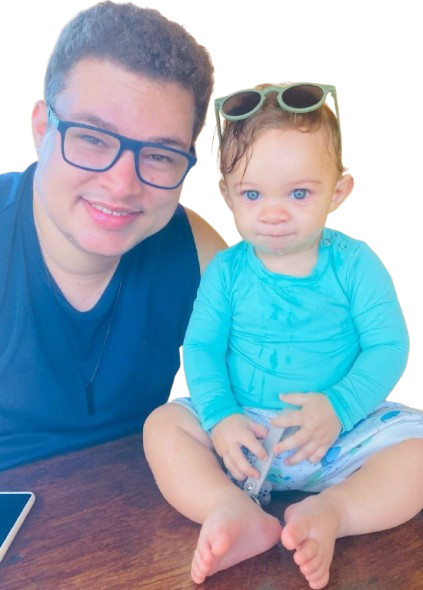
\includegraphics[width=2cm]{diego.png}
\end{wrapfigure}\noindent
Nascido na seca cidade de Caculé, no sertão da Bahia, Diego Lima Bomfim peregrinou por considerável parte do Estado: fez o ensino médio e técnico na fria Vitória da Conquista, formou-se em Matemática na calorosa São Salvador --- onde também concluiu o mestrado e iniciou o doutorado --- e é, desde 2024, professor efetivo do Instituto Federal de Educação, Ciência e Tecnologia da Bahia (IFBA), na chuvosa cidade de Valença. Medalhista da OBMEP na juventude, tornou-se pai no mesmo ano em que assumiu o cargo de professor e agora se divide entre equações e as traquinagens de Vinicius, um menino sapeca, curioso, cheio de energia e imaginação -- típico de um episódio de {\it Os Anjinhos}. Flamenguista de coração e fã de esportes em geral, acredita que a matemática, assim como o futebol, é melhor quando compartilhada.

\end{document}
